\documentclass[11pt,aspectratio=169]{beamer}

% Packages
\usepackage{mathtools}
\usepackage{hyperref}
\usepackage{setspace}
\usepackage{tikz}
\usetikzlibrary{positioning}
\usepackage{ragged2e}
\usepackage{nicematrix}
\usepackage[compatibility=false]{caption}
\usepackage[framemethod=tikz]{mdframed}

% Colored boxes
\usepackage{tcolorbox}
\tcbsetforeverylayer{autoparskip} % Removes unwanted vertical space

% Theme
\usetheme{metropolis}
\metroset{subsectionpage=progressbar,sectionpage=none}
\setbeamertemplate{theorems}[numbered]

\usepackage{fontspec}
\defaultfontfeatures{LetterSpace=30}
\usepackage{microtype}

% Prefer flexible inter-word spacing over splitting words across lines.
\tolerance=1
\emergencystretch=\maxdimen
\hyphenpenalty=10000
\hbadness=10000


% Code
\usepackage{listings}
% Custom colors
\definecolor{codegreen}{rgb}{0,0.6,0}
\definecolor{codegray}{rgb}{0.5,0.5,0.5}
\definecolor{codepurple}{rgb}{0.58,0,0.82}
\definecolor{backcolour}{rgb}{0.95,0.95,0.92}
\definecolor{light-gray}{gray}{0.95}
% Python style for highlighting
\newcommand\pythonstyle{\lstset{
		backgroundcolor=\color{white},
		language=Python,
		basicstyle=\ttfamily\footnotesize,
		morekeywords={self},              % Add keywords here
		keywordstyle=\color{blue},
		stringstyle=\footnotesize\color{deepgreen},
		commentstyle=\color{codegreen},
		showstringspaces=false,
		frame=tb,
		numbers=left,
		numbersep=5pt,
		numberstyle=\tiny\color{gray},
		columns=fullflexible,
		numbersep=5pt,
		aboveskip=1em,
		showtabs=false,
		tabsize=2,
		gobble=3
	}}

% Python environment
\lstnewenvironment{python}[1][]
{
	\pythonstyle
	\lstset{#1}
}
{}
% Python for inline
\newcommand\pythoninline[1]{{\pythonstyle\lstinline!#1!}}

% Tables and justification
\newcommand{\ra}[1]{\renewcommand{\arraystretch}{#1}}
\justifying

% Subfigures
\setbeamertemplate{caption}[numbered]
\usepackage[caption=false,font=footnotesize]{subfig}

% Colors
\setbeamercolor{uppercolgreen}{fg=white,bg=green!35}
\setbeamercolor{lowercolgreen}{fg=black,bg=green!10}
\setbeamercolor{uppercolred}{fg=white,bg=red!35}
\setbeamercolor{lowercolred}{fg=black,bg=red!10}
\setbeamercolor{uppercolblue}{fg=white,bg=blue!35}
\setbeamercolor{lowercolblue}{fg=black,bg=blue!10}
\definecolor{darkred}{rgb}{0.55, 0.0, 0.0}
\definecolor{darkpastelblue}{rgb}{0.47, 0.62, 0.8}
\definecolor{darkcerulean}{rgb}{0.03, 0.27, 0.49}
\definecolor{darkgreen}{rgb}{0.0, 0.55, 0.0}
\definecolor{deepblue}{rgb}{0,0,0.5}
\definecolor{deepred}{rgb}{0.6,0,0}
\definecolor{deepgreen}{rgb}{0,0.5,0}

% Matrix size
\usepackage{stackengine}
\stackMath
\def\sss{\scriptstyle \color{gray}}
\setstackgap{L}{12pt}
\def\stacktype{L}

% Mathematical commands
\newcommand{\vc}[1]{\boldsymbol{\mathbf{#1}}}
\newcommand{\pr}[1]{{#1\,}'}
\newcommand{\idx}[2]{{\color{darkpastelblue}[}#1{\color{darkpastelblue}]_{#2}}}
\newcommand{\shape}[2]{\stackunder{#1}{\sss #2}}
\DeclareMathOperator*{\argmax}{arg\,max}
\DeclareMathOperator*{\argmin}{arg\,min}

% Style commands
\newcommand{\myalert}[1]{{\color{darkred}\textbf{#1}}}

% White frame (for images)
\newenvironment{whiteframe}[1]{
	\setbeamercolor{background canvas}{bg=white}
	\begin{frame}{#1}
		}{
	\end{frame}
}

\setbeamerfont{frametitle}{size=\normalsize}
\setbeamertemplate{frametitle}[default][right]
{
}
%\setbeamercolor{frametitle}{fg=white,bg=black!75}

% No headline frame
\makeatletter
\newenvironment{noheadline}{
	\setbeamertemplate{headline}{}
	\addtobeamertemplate{frametitle}{\vspace*{-3.5\baselineskip}}{}
}{}
\makeatother

% Lists
\setbeamertemplate{itemize items}[triangle]

% Footnotes
\setbeamertemplate{footnote}%
{%
	\parindent 1.5em\noindent%
	\justifying\setstretch{0.7}%
	\hbox to 1em{\hfil\insertfootnotemark}\begin{scriptsize}\insertfootnotetext\end{scriptsize}\par%
}

% Footnote without number
\newcommand\blfootnote[1]{%
	\begingroup
	\renewcommand\thefootnote{}\footnote[frame]{\noindent#1}%
	\addtocounter{footnote}{-1}%
	\endgroup
}

% Slide sources: set in the frame footer beside the page number, so they
% take no room from the content. Zero height keeps the footline unchanged.
% Global, because the footline is typeset outside the frame's group; each
% frame starts empty.
\newcommand{\insertslidesource}{}
\newcommand{\SlideSource}[1]{\gdef\insertslidesource{#1}}
\AddToHook{env/frame/begin}{\gdef\insertslidesource{}}
\setbeamertemplate{frame footer}{%
	\ifx\insertslidesource\empty\else
		\smash{\parbox[b]{0.88\textwidth}{\raggedright\scriptsize\color{black!60}\insertslidesource}}%
	\fi}

% Theorems
\newcommand*{\theorembreak}{\usebeamertemplate{theorem end}\framebreak\usebeamertemplate{theorem begin}}
\newcounter{theo}[section]\setcounter{theo}{0}
\renewcommand{\thetheo}{\arabic{section}.\arabic{theo}}

\newenvironment{theo}[2][]{%
	\refstepcounter{theo}%
	\ifstrempty{#1}%
	{\mdfsetup{%
			frametitle={%
					\tikz[baseline=(current bounding box.east),outer sep=0pt]
					\node[anchor=east,rectangle,fill=red!10]
					{\strut Theorem~\thetheo};}}
	}%
	{\mdfsetup{%
			frametitle={%
					\tikz[baseline=(current bounding box.east),outer sep=0pt]
					\node[anchor=east,rectangle,fill=red!10]
					{\strut Theorem~\thetheo:~#1};}}%
	}%
	\mdfsetup{innertopmargin=5pt,linecolor=red!10,%
		linewidth=2pt,topline=true,%
		frametitleaboveskip=\dimexpr-\ht\strutbox\relax
	}
	\begin{mdframed}[]\relax%
		\label{#2}}{\end{mdframed}}

% Shared content names each box group; the course controls its height.
\tcbset{courseheight/.style 2 args={height=#2}}

\usetikzlibrary{arrows.meta,calc,decorations.pathreplacing}
\graphicspath{{assets/}{../../shared/assets/}}

\usepackage{annotate-equations}
\usepackage{pgfplots}
\pgfplotsset{compat=1.18}

% Written by Claude (2026-11-12): second deck of the Transformer refresh (plan
% in the vault's NNDS Slide Refresh Log, 2026-11-12). Built block by block;
% this file starts with the first block, the modern transformer block.

% Colors and diagram styles shared by the two transformer decks
% (Lecture_transformers.tex and Lecture_modern_transformers.tex).

% Query, key and value colors, reused in equations and figures (local to NNDS
% for now; move to shared/style/content.tex if NN adopts them).
\colorlet{qcolor}{drawviolet!80!black}
\colorlet{kcolor}{draworange!85!black}
\colorlet{vcolor}{darkcerulean}
\newcommand{\qc}[1]{{\color{qcolor}#1}}
\newcommand{\kc}[1]{{\color{kcolor}#1}}
\newcommand{\vcl}[1]{{\color{vcolor}#1}}

% Block-diagram styles, as in shared/slides/mlps.tex and the deeper-models deck.
\tikzset{
    nnblock/.style={
            draw=drawblue, fill=drawblue_l!25!white, rounded corners=2pt,
            minimum width=1.25cm, minimum height=0.65cm,
            inner sep=5pt, font=\small
        },
    nnother/.style={nnblock, draw=drawgreen, fill=drawgreen_l!25!white},
    nnmerge/.style={
            circle, draw=drawgray, fill=white,
            minimum size=0.55cm, inner sep=1pt, font=\small
        },
    nnedge/.style={->, thick, draw=drawgray}
}

% Full-size diagram styles for the transformer figures: arrows as in the
% attention figures (Stealth tips, gray), boxes at normal size.
\tikzset{
    tfarr/.style={-{Stealth[length=5pt]}, drawgray, line width=0.6pt},
    tfblk/.style={draw=drawblue, fill=drawblue_l!60, rounded corners=2pt,
            minimum height=0.75cm, minimum width=1.9cm, inner sep=4pt, font=\small},
    tfnorm/.style={tfblk, draw=drawgreen, fill=drawgreen_l!70},
    tfsum/.style={circle, draw=drawgray, fill=white, minimum size=0.45cm, inner sep=0pt, font=\small},
    tflab/.style={font=\scriptsize, text=black!60},
}


\begin{document}

{\usebackgroundtemplate{\tikz\node[opacity=0.4,inner sep=0]{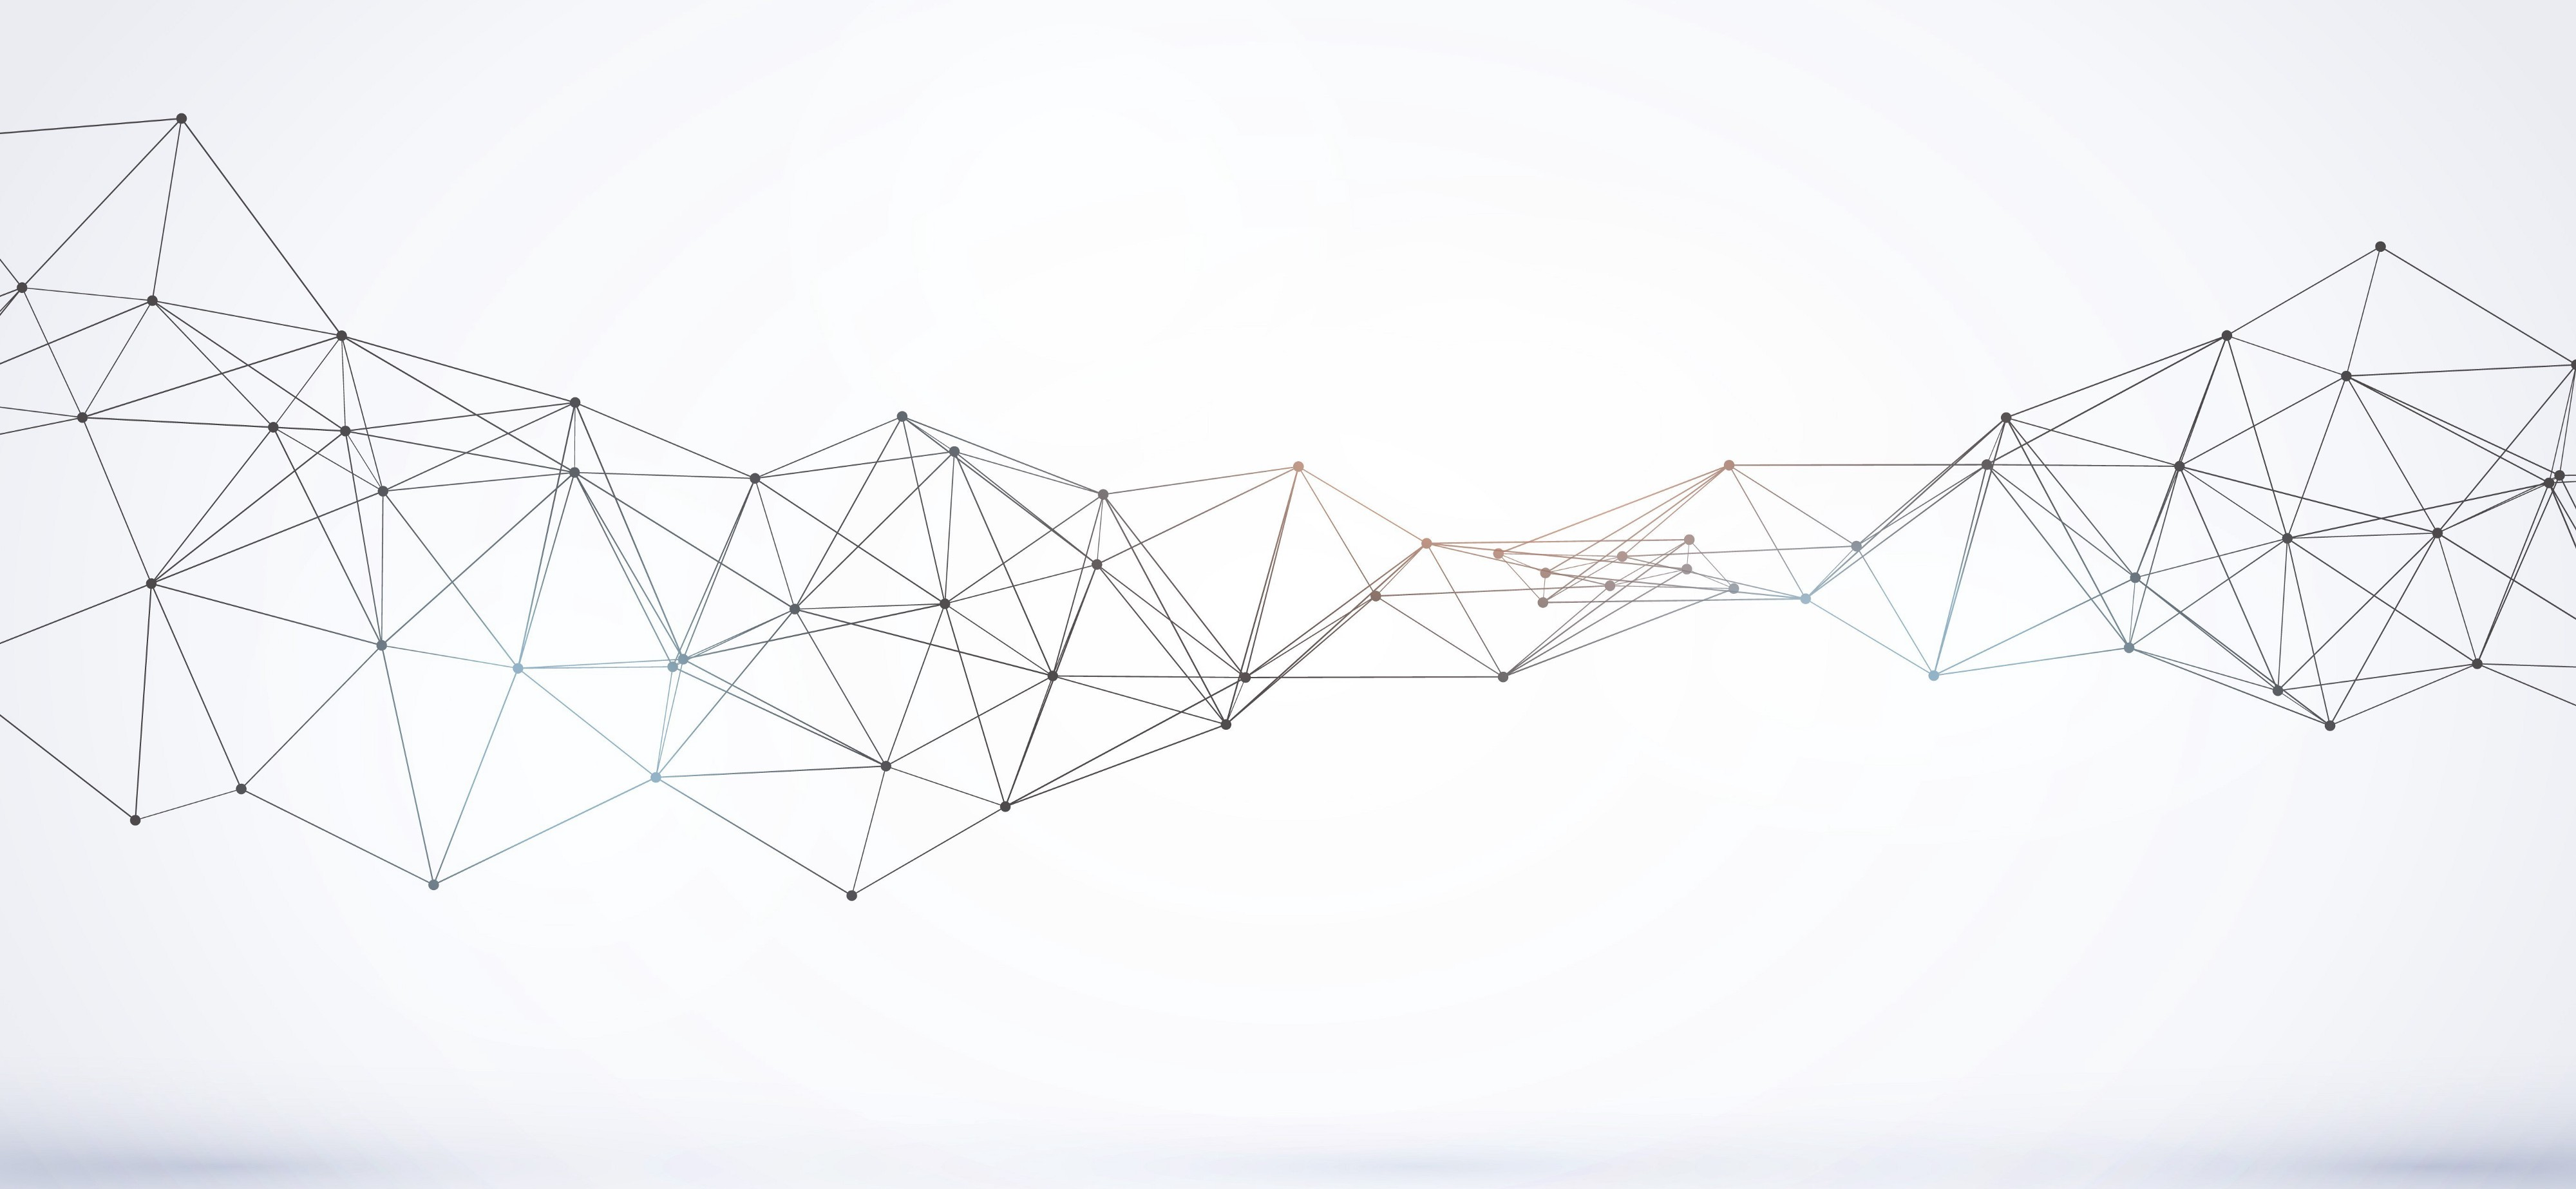
\includegraphics[width=\paperwidth,height=\paperheight]{images/header}};}%
\begin{frame}[plain]
    \vspace{0.5cm}
    \title{\large \begin{spacing}{1.0}Neural Networks for Data Science\end{spacing}\vspace{0.25em}
        \normalsize \begin{spacing}{1.0}\textbf{Master's Degree in Data Science}\end{spacing}\vspace{0.5em}}
    \subtitle{\Large \textbf{Modern transformers}}
    \date{
        {
\includegraphics[scale=0.8]{images/Uniroma1}}
    }
    \author{
        \setlength{\tabcolsep}{2pt}
        \begin{tabular}{rl}
            \textbf{Lecturer}: & S. Scardapane \\
        \end{tabular}
    }\titlepage
\end{frame}
}

\part{1}

\section{The modern transformer block}
\subsection{Normalization, positions and the MLP}

\begin{frame}{From 2017 to today}
    \setlength{\parskip}{5pt}

    Modern language models are still built by stacking transformer blocks,
    but most components inside the block have changed since the 2017 design:

    \centering
    \begin{tikzpicture}[x=1.17cm, y=1cm,
            pb/.style={tfblk, minimum width=1.5cm, minimum height=0.6cm},
            pn/.style={tfnorm, minimum width=1.5cm, minimum height=0.6cm},
            skip/.style={tfarr, drawgray!70},
            ttl/.style={font=\small\bfseries, anchor=west, text=black!70},
        ]
        % 2017: X -> MHA -> + -> LN -> MLP -> + -> LN
        \node[ttl] (t17) at (-0.2,1.05) {2017};
        \node[tflab, anchor=base west] at (t17.base east) {positional embeddings added to $\vc{X}$, biases in every layer};
        \node[font=\small] (x) at (0,0) {$\vc{X}$};
        \node[pb] (a) at (1.6,0) {MHA};
        \node[tfsum] (m1) at (3.1,0) {$+$};
        \node[pn] (n1) at (4.6,0) {LayerNorm};
        \node[pb] (f) at (6.6,0) {MLP};
        \node[tfsum] (m2) at (8.1,0) {$+$};
        \node[pn] (n2) at (9.6,0) {LayerNorm};
        \node[font=\small] (y) at (11.1,0) {$\vc{H}$};
        \draw[tfarr] (x) -- (a); \draw[tfarr] (a) -- (m1); \draw[tfarr] (m1) -- (n1);
        \draw[tfarr] (n1) -- (f); \draw[tfarr] (f) -- (m2); \draw[tfarr] (m2) -- (n2);
        \draw[tfarr] (n2) -- (y);
        \draw[skip] (0.6,0) -- (0.6,0.65) -| (m1);
        \draw[skip] (5.6,0) -- (5.6,0.65) -| (m2);
        \fill[drawgray] (0.6,0) circle (1.3pt); \fill[drawgray] (5.6,0) circle (1.3pt);
        \node[tflab, below=3pt] at (f.south) {ReLU};

        % Today: X -> RMSNorm -> MHA -> + -> RMSNorm -> MLP -> +
        \begin{scope}[yshift=-2.0cm]
            \node[ttl] (tnow) at (-0.2,1.05) {Today};
            \node[tflab, anchor=base west] at (tnow.base east) {no biases};
            \node[font=\small] (x) at (0,0) {$\vc{X}$};
            \node[pn] (n1) at (1.6,0) {RMSNorm};
            \node[pb] (a) at (3.6,0) {MHA};
            \node[tfsum] (m1) at (5.1,0) {$+$};
            \node[pn] (n2) at (6.6,0) {RMSNorm};
            \node[pb] (f) at (8.6,0) {MLP};
            \node[tfsum] (m2) at (10.1,0) {$+$};
            \node[font=\small] (y) at (11.1,0) {$\vc{H}$};
            \draw[tfarr] (x) -- (n1); \draw[tfarr] (n1) -- (a); \draw[tfarr] (a) -- (m1);
            \draw[tfarr] (m1) -- (n2); \draw[tfarr] (n2) -- (f); \draw[tfarr] (f) -- (m2);
            \draw[tfarr] (m2) -- (y);
            \draw[skip] (0.6,0) -- (0.6,0.65) -| (m1);
            \draw[skip] (5.6,0) -- (5.6,0.65) -| (m2);
            \fill[drawgray] (0.6,0) circle (1.3pt); \fill[drawgray] (5.6,0) circle (1.3pt);
            \node[tflab, below=3pt] at (n1.south) {pre-norm};
            \node[tflab, below=3pt] at (a.south) {RoPE, (QK-norm)};
            \node[tflab, below=3pt] at (f.south) {SwiGLU};
        \end{scope}
    \end{tikzpicture}
    \par\vspace{0.4em}
    \justifying

    Most recent decoder models (e.g., Llama~3, Qwen3) use the second block,
    with minor variations.

    \SlideSource{\href{https://arxiv.org/abs/1706.03762}{Vaswani et al. (2017)}; \href{https://arxiv.org/abs/2407.21783}{Grattafiori et al., Llama 3 (2024)}; \href{https://arxiv.org/abs/2505.09388}{Yang et al., Qwen3 (2025)}.}

\end{frame}

\begin{frame}{Changes we have already seen}
    \setlength{\parskip}{6pt}

    We have already seen three of these changes in the previous lectures:
    \[
        \vc{H}'=\vc{X}+\operatorname{MHA}(\operatorname{RMSNorm}(\vc{X})) \,,
        \qquad
        \vc{H}=\vc{H}'+\operatorname{MLP}(\operatorname{RMSNorm}(\vc{H}')) \,.
    \]
    \begin{itemize}
        \setlength{\itemsep}{5pt}
        \item \myalert{Pre-normalization}: the residual path carries $\vc{X}$
              (and its gradient) unchanged through the stack, with an
              additional normalization before the classifier.
        \item \myalert{RMSNorm} instead of LayerNorm: we only divide by the
              norm, without subtracting the mean (the previous linear layer
              can learn it).
        \item \myalert{RoPE} instead of additive positional embeddings: the
              \qc{queries} and \kc{keys} are rotated in every MHA layer, so
              that the scores depend on the relative position $t'-t$.
    \end{itemize}

    \SlideSource{\href{https://arxiv.org/abs/2002.04745}{Xiong et al. (2020)}; \href{https://arxiv.org/abs/1910.07467}{Zhang and Sennrich (2019)}; \href{https://arxiv.org/abs/2104.09864}{Su et al., RoFormer (2024)}.}

\end{frame}

\begin{frame}{The MLP: SwiGLU}
    \setlength{\parskip}{5pt}

    Most recent models replace the two-layer MLP with the \myalert{SwiGLU}
    layer we saw in the MLP lecture, in which a second projection of the
    input acts as a gate:

    \begin{center}
        \begin{tikzpicture}
			\node (x) at (0,0) {$\vc{x}$};
\node[nnblock] (u) at (1.8,0.65) {$\vc{W}_u$};
\node[nnother] (g) at (1.8,-0.65) {$\vc{W}_g$};
\node[nnother] (phi) at (3.5,-0.65) {$\phi$};
\node[nnmerge] (m) at (5,0) {$\odot$};
\node[nnblock] (o) at (6.5,0) {$\vc{W}_o$};
\node (y) at (7.9,0) {$\vc{y}$};

			\draw[nnedge] (x)|-(u);
\draw[nnedge] (x)|-(g);
\draw[nnedge] (g)--(phi);
\draw[nnedge] (u.east)--(5,0.65)--(m.north);
\draw[nnedge] (phi.east)-|(m.south);
\draw[nnedge] (m)--(o);
\draw[nnedge] (o)--(y);

		\end{tikzpicture}

    \end{center}
    \vspace{-0.8em}
    \[
        \vc{y}=\vc{W}_o\left[(\vc{W}_u\vc{x})\odot\operatorname{SiLU}(\vc{W}_g\vc{x})\right] ,
        \qquad \vc{W}_u,\vc{W}_g\in\mathbb{R}^{M\times D},\;\;
        \vc{W}_o\in\mathbb{R}^{D\times M} \,.
    \]
    We now have three matrices instead of two. To keep the $8D^2$ parameters
    of the original MLP, the hidden size is reduced from $4D$ to
    $M=\tfrac{2}{3}\cdot 4D$, so that $3DM=8D^2$ (e.g., $D=4096$ and
    $M=11008$ in Llama~2 7B). In this way, the block still has
    \myalert{$12D^2$~parameters}.

    \SlideSource{\href{https://arxiv.org/abs/2002.05202}{Shazeer (2020)}; \href{https://arxiv.org/abs/2302.13971}{Touvron et al., LLaMA (2023)}.}

\end{frame}

\subsection{Biases, QK-norm and parallel blocks}

\begin{frame}{Removing the biases}
    \setlength{\parskip}{6pt}

    The original block has a bias in every linear layer and in every
    LayerNorm. Most recent language models remove all of them, for a few
    reasons:

    \begin{itemize}
        \setlength{\itemsep}{4pt}
        \item They are a tiny fraction of the model: in GPT-2 (small), biases
              and LayerNorm parameters are about $0.12$M out of $124$M.
        \item Some of them have no effect. For example, a bias $\vc{b}$ on the
              keys adds the same value $\qc{\vc{q}_t^{\top}}\vc{b}$ to all the
              scores of token $t$, which is ignored by the softmax:
              \[
                  \operatorname{softmax}_{t'}\big(\qc{\vc{q}_t^{\top}}(\kc{\vc{k}_{t'}}+\vc{b})\big)
                  =\operatorname{softmax}_{t'}\big(\qc{\vc{q}_t^{\top}}\kc{\vc{k}_{t'}}\big) \,.
              \]
        \item Empirically, training large models is more stable without them.
    \end{itemize}

    RMSNorm only keeps the gain $\vc{\gamma}$ which, as discussed in the
    lecture on deeper models, can be absorbed by the next linear layer: \mbox{$\vc{W}(\vc{\gamma}\odot\vc{u})=(\vc{W}\operatorname{diag}(\vc{\gamma}))\vc{u}$}.

    \SlideSource{\href{https://arxiv.org/abs/2204.02311}{Chowdhery et al., PaLM (2023)}, JMLR.}

\end{frame}

\begin{frame}{Normalizing queries and keys}
    \setlength{\parskip}{6pt}

    Dividing by $\sqrt{D_k}$ keeps the scores small at initialization, but
    not necessarily during training: if queries and keys grow, a single large
    score can saturate the softmax.

    \myalert{Q/K normalized} variants add a normalization over the keys and
    queries before computing the scores. In the simplest version:
    \[
        s_{t,t'}=\eqnmarkbox[drawblue]{gain}{g}\;
        \frac{\qc{\vc{q}_t^{\top}}\kc{\vc{k}_{t'}}}{\lVert\qc{\vc{q}_t}\rVert\,\lVert\kc{\vc{k}_{t'}}\rVert} \,.
    \]
    \annotate[yshift=-0.6em]{below,left}{gain}{trainable scale, replaces $1/\sqrt{D_k}$}
    \vspace{0.4em}

    The score is now a cosine similarity, bounded in $[-g,g]$. Recent models
    (e.g., ViT-22B, Gemma~3, Qwen3) keep the fixed scaling and apply a
    LayerNorm or RMSNorm (with its own gain) to queries and keys, before RoPE
    (rotations do not change the norm).

    \SlideSource{\href{https://arxiv.org/abs/2010.04245}{Henry et al. (2020)}; \href{https://arxiv.org/abs/2302.05442}{Dehghani et al., ViT-22B (2023)}; \href{https://arxiv.org/abs/2503.19786}{Gemma 3 (2025)}; \href{https://arxiv.org/abs/2505.09388}{Qwen3 (2025)}.}

\end{frame}

\begin{frame}{Parallel blocks}
    \setlength{\parskip}{5pt}

    \myalert{Parallel} variants perform the MHA and MLP operations in
    parallel, on the same normalized input:
    $\vc{H}=\vc{X}+\operatorname{MHA}(\operatorname{Norm}(\vc{X}))+\operatorname{MLP}(\operatorname{Norm}(\vc{X}))$.

    \vspace{0.2em}
    \centering
    \begin{tikzpicture}[x=1.17cm, y=1cm,
            pb/.style={tfblk, minimum width=1.5cm, minimum height=0.6cm},
            pn/.style={tfnorm, minimum width=1.5cm, minimum height=0.6cm},
            skip/.style={tfarr, drawgray!70},
        ]
        \node[font=\small] (x) at (0,0) {$\vc{X}$};
        \node[pn] (n) at (2.0,0) {Norm};
        \node[pb] (a) at (4.6,0) {MHA};
        \node[pb] (f) at (4.6,-1.0) {MLP};
        \node[tfsum] (m) at (6.9,0) {$+$};
        \node[font=\small] (y) at (8.3,0) {$\vc{H}$};
        \draw[tfarr] (x) -- (n);
        \draw[tfarr] (n) -- (a);
        \draw[tfarr] (a) -- (m);
        \draw[tfarr] (3.3,0) |- (f.west);
        \draw[tfarr] (f.east) -| (m.south);
        \draw[tfarr] (m) -- (y);
        \draw[skip] (0.7,0) -- (0.7,0.65) -| (m);
        \fill[drawgray] (0.7,0) circle (1.3pt); \fill[drawgray] (3.3,0) circle (1.3pt);
    \end{tikzpicture}
    \par\vspace{0.3em}
    \justifying

    In this way, the initial and final projections of the MLP and MHA layers
    can be fused, each in a single matrix product.

    PaLM reports about $15\%$ faster training, with no loss in quality for
    its larger models. However, most open language models (e.g., Llama, Qwen,
    Gemma) still use the sequential block.

    \SlideSource{\href{https://arxiv.org/abs/2302.05442}{Dehghani et al., ViT-22B (2023)}, ICML; \href{https://arxiv.org/abs/2204.02311}{Chowdhery et al., PaLM (2023)}, JMLR.}

\end{frame}

\begin{frame}[fragile]{A modern block in code}
    \setlength{\parskip}{5pt}

    \begin{python}[gobble=8,aboveskip=2pt,belowskip=4pt]
        def forward(self, x):                                  # x: (B, T, D)
            B, T, D = x.shape
            q, k, v = (z.view(B, T, self.h, -1).transpose(1, 2)   # (B, h, T, D/h)
                       for z in self.qkv(self.norm1(x)).chunk(3, -1))
            a = F.scaled_dot_product_attention(
                    rope(q), rope(k), v, is_causal=True)
            x = x + self.out(a.transpose(1, 2).reshape(B, T, D))
            z = self.norm2(x)
            return x + self.down(self.up(z) * F.silu(self.gate(z)))
    \end{python}

    Here, the two normalizations are \pythoninline{nn.RMSNorm(D)}, all other
    layers are \pythoninline{nn.Linear} with \pythoninline{bias=False}, and
    \pythoninline{rope} is the function we wrote in the last lecture. In
    total, the block has $12D^2+2D$ parameters (the $2D$ are the two gains).

\end{frame}

\section{Generating text}
\subsection{The KV cache}

\begin{frame}{Prefill and decode}
    \setlength{\parskip}{6pt}

    Generating the answer to a prompt of $T_p$ tokens happens in two phases:
    \begin{itemize}
        \setlength{\itemsep}{4pt}
        \item \myalert{Prefill}: a single forward pass over the entire
              prompt, computed in parallel as during training. The last
              prediction gives us the first new token.
        \item \myalert{Decode}: one forward pass for every new token, which
              must attend to all the previous ones.
    \end{itemize}

    Because of the causal mask, a new token does not change the hidden states
    of the previous ones (in any layer), so recomputing their \kc{keys} and
    \vcl{values} at every step is wasteful.

    \begin{tcolorbox}[nndsgreen]
        \textbf{\color{darkgreen}KV cache}: in every layer, we store the
        \kc{keys} and \vcl{values} of all past tokens, and we compute
        $\qc{\vc{q}}$, $\kc{\vc{k}}$, $\vcl{\vc{v}}$ only for the new token.
    \end{tcolorbox}

\end{frame}

\begin{whiteframe}{The KV cache}
    \setlength{\abovecaptionskip}{6pt}

    \begin{figure}
        \centering
        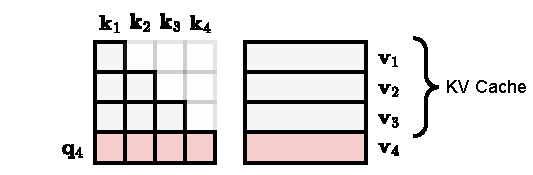
\includegraphics[width=0.75\textwidth]{images/transformers/book/kv_cache.pdf}
        \caption{Decoding the fourth token with a KV cache. We only need the
            last row of the attention matrix (which has no masked entries): the
            new query $\qc{\vc{q}_4}$ is compared with
            $\kc{\vc{k}_1},\ldots,\kc{\vc{k}_4}$, of which only $\kc{\vc{k}_4}$
            and $\vcl{\vc{v}_4}$ are new. For each layer, the cost of a step goes
            from $\mathcal{O}(tD^2+t^2D)$ to $\mathcal{O}(D^2+tD)$.}
    \end{figure}

\end{whiteframe}

\begin{frame}[fragile]{The KV cache in code}
    \setlength{\parskip}{6pt}

    Inside each attention layer, \pythoninline{x} now contains only the new
    tokens:

    \begin{python}[gobble=8,aboveskip=2pt,belowskip=2pt]
        q, k, v = self.qkv_heads(x, start)            # RoPE from position start
        if start > 0:                                 # decode: append to the cache
            k = torch.cat([self.k_cache, k], dim=2)
            v = torch.cat([self.v_cache, v], dim=2)
        self.k_cache, self.v_cache = k, v
        a = F.scaled_dot_product_attention(q, k, v, is_causal=(start == 0))
    \end{python}

    Generation is a single prefill call, followed by one call for each new
    token (here, with greedy decoding):

    \begin{python}[gobble=8,aboveskip=2pt,belowskip=2pt]
        logits = model(prompt, start=0)               # prefill: fills the caches
        for t in range(T_p, T_p + n):
            z = logits[:, -1].argmax(-1, keepdim=True)
            logits = model(z, start=t)                # decode: one token
    \end{python}

\end{frame}

\begin{frame}{How large is the KV cache?}
    \setlength{\parskip}{6pt}

    \begin{columns}[T,onlytextwidth]
        \begin{column}{0.46\textwidth}
            \setlength{\parskip}{6pt}
            For each of the $N$ layers, every token stores a \kc{key} and a
            \vcl{value} of size $D$. With $b$ bytes per number, the total is:
            \[
                \text{cache}=2\cdot N\cdot D\cdot T\cdot b \text{ bytes.}
            \]
            For example, Llama~2 7B ($N=32$, $D=4096$, $16$ bits) needs
            $0.5$\,MB per token, or $2$\,GB for a sequence of $T=4096$ tokens.
        \end{column}
        \begin{column}{0.5\textwidth}
            \centering
            \begin{tikzpicture}
                \begin{axis}[
                        width=\linewidth, height=0.56\textheight,
                        ybar stacked, bar width=16pt, ymin=0, ymax=90,
                        symbolic x coords={1,4,16,32}, xtick=data,
                        xlabel={Sequences in the batch}, ylabel={Memory (GB)},
                        label style={font=\small}, tick label style={font=\small},
                        axis lines=left, axis line style={drawgray},
                        enlarge x limits=0.18, clip=false,
                        legend style={font=\scriptsize, draw=none, fill=none, at={(0.03,0.82)}, anchor=north west},
                        legend cell align=left,
                    ]
                    \addplot[fill=drawblue_l, draw=drawblue] coordinates {(1,13.5) (4,13.5) (16,13.5) (32,13.5)};
                    \addplot[fill=draworange!70, draw=draworange] coordinates {(1,2.1) (4,8.6) (16,34.4) (32,68.7)};
                    \legend{Weights, KV cache}
                    \draw[drawred, dashed, thick] (rel axis cs:0,0.889) -- (rel axis cs:1,0.889)
                        node[anchor=south east, font=\scriptsize, text=drawred] {80 GB GPU};
                \end{axis}
            \end{tikzpicture}
        \end{column}
    \end{columns}

    \medskip
    Since every decoding step reads the entire cache, its size limits how
    many sequences we can serve at once. Next, we reduce it by sharing
    \kc{keys} and \vcl{values} among heads.

    \SlideSource{\href{https://arxiv.org/abs/2307.09288}{Touvron et al., Llama 2 (2023)}; \href{https://arxiv.org/abs/2211.05102}{Pope et al., Efficiently scaling transformer inference (2023)}.}

\end{frame}

\section{Smaller caches}
\subsection{Sharing keys and values among heads}

\begin{frame}{Multi-query and grouped-query attention}
    \setlength{\parskip}{6pt}

    In MHA, we need to cache the \kc{keys} and \vcl{values} of all $h$ heads.
    Two common variants keep the $h$ \qc{query} heads, but reduce the number
    of key/value heads:
    \begin{itemize}
        \setlength{\itemsep}{3pt}
        \item \myalert{Multi-query attention} (MQA): all query heads share a
              single key head and a single value head.
        \item \myalert{Grouped-query attention} (GQA): the query heads are
              split into $G$ groups, and each group shares one key and one value
              head.
    \end{itemize}

    \vspace{0.3em}
    \centering
    % Written by Claude (2026-11-13): query heads and the key/value heads they
% read, for MHA, GQA (G = 2) and MQA, with h = 8 query heads.
\begin{tikzpicture}[x=0.92cm, y=1cm,
        hd/.style={minimum size=0.32cm, inner sep=0pt, line width=0.6pt},
        qh/.style={hd, draw=qcolor, fill=qcolor!25},
        kh/.style={hd, draw=kcolor, fill=kcolor!30},
        vh/.style={hd, draw=vcolor, fill=vcolor!25},
        ln/.style={drawgray, line width=0.5pt},
        ttl/.style={font=\small\bfseries, text=black!75},
        rowlab/.style={font=\scriptsize, text=black!60, anchor=east},
    ]
    % #1: x offset, #2: number of key/value heads
    \newcommand{\kvpanel}[3]{%
        \begin{scope}[xshift=#1cm]
            \pgfmathsetmacro{\gs}{8/#2}
            \foreach \i in {0,...,7} {
                    \node[qh] (q\i) at ({\i*0.42},1.5) {};
                }
            \foreach \g in {1,...,#2} {
                    \pgfmathsetmacro{\xc}{((\g-1)*\gs + (\gs-1)/2)*0.42}
                    \node[kh] (k\g) at (\xc,0.5) {};
                    \node[vh] (v\g) at (\xc,0.0) {};
                    \pgfmathtruncatemacro{\first}{(\g-1)*\gs}
                    \pgfmathtruncatemacro{\last}{\g*\gs-1}
                    \foreach \i in {\first,...,\last} {
                            \draw[ln] (q\i.south) -- (k\g.north);
                        }
                }
            \node[ttl] at (1.47,2.1) {#3};
        \end{scope}
    }
    \kvpanel{0}{8}{Multi-head ($G=h$)}
    \kvpanel{4.4}{2}{Grouped-query ($G=2$)}
    \kvpanel{8.8}{1}{Multi-query ($G=1$)}
    \node[rowlab] at (-0.3,1.5) {\qc{queries}};
    \node[rowlab] at (-0.3,0.5) {\kc{keys}};
    \node[rowlab] at (-0.3,0.0) {\vcl{values}};
\end{tikzpicture}


    \SlideSource{\href{https://arxiv.org/abs/1911.02150}{Shazeer (2019)}; \href{https://arxiv.org/abs/2305.13245}{Ainslie et al., GQA (2023)}, EMNLP.}

\end{frame}

\begin{frame}[fragile]{Grouped-query attention in practice}
    \setlength{\parskip}{6pt}

    With GQA, the cache goes from $2hD_k$ to $2GD_k$ numbers per token and
    layer. MQA can lose some quality, while GQA is close to MHA in quality
    and to MQA in speed.

    For example, Llama~3 8B has the same $N=32$ and $D=4096$ as Llama~2 7B,
    but $G=8$ key/value heads for $h=32$ query heads: $128$\,KB per token
    instead of $512$\,KB.

    In code, we only change the number of key and value heads:
    \begin{python}[gobble=8,aboveskip=2pt,belowskip=2pt]
        q = self.wq(x).view(B, T, h, -1).transpose(1, 2)    # (B, h, T, D_k)
        k = self.wk(x).view(B, T, G, -1).transpose(1, 2)    # (B, G, T, D_k)
        v = self.wv(x).view(B, T, G, -1).transpose(1, 2)    # (B, G, T, D_k)
        a = F.scaled_dot_product_attention(q, k, v, is_causal=True,
                                           enable_gqa=True)   # each k, v serves h/G heads
    \end{python}

    An MHA model can also be converted to GQA by averaging the key and value
    heads of each group, followed by a short additional training.

    \SlideSource{\href{https://arxiv.org/abs/2305.13245}{Ainslie et al., GQA (2023)}, EMNLP; \href{https://arxiv.org/abs/2407.21783}{Grattafiori et al., Llama 3 (2024)}.}

\end{frame}

\begin{frame}{Multi-head latent attention (MLA)}
    \setlength{\parskip}{6pt}

    In MLA, each token stores instead a single compressed vector, from which
    every head reconstructs its key and value:
    \[
        \eqnmarkbox[drawblue]{lat}{\vc{c}_t=\vc{W}_c\vc{x}_t} \,, \qquad
        \kc{\vc{k}_{t,i}=\vc{W}_{k,i}\vc{c}_t} \,, \qquad
        \vcl{\vc{v}_{t,i}=\vc{W}_{v,i}\vc{c}_t} \,.
    \]
    \annotate[yshift=-0.5em]{below,left}{lat}{cached, size $d_c\ll 2hD_k$}
    \vspace{0.6em}

    We never compute the keys explicitly, since $\qc{\vc{q}_{t,i}^{\top}}\vc{W}_{k,i}\vc{c}_{t'}=(\vc{W}_{k,i}^{\top}\qc{\vc{q}_{t,i}})^{\top}\vc{c}_{t'}$
    and $\vc{W}_{k,i}$ can be merged into the query projection ($\vc{W}_{v,i}$
    into the output one). RoPE would break this trick, so MLA adds a small
    key with RoPE, shared by all heads.

    In DeepSeek-V2 and V3, this is $512+64=576$ numbers per token and layer,
    against $2hD_k=32{,}768$ for MHA (equivalent to GQA with $2.25$ groups),
    with better quality than MHA in their experiments.

    \SlideSource{\href{https://arxiv.org/abs/2405.04434}{DeepSeek-AI, DeepSeek-V2 (2024)}; \href{https://arxiv.org/abs/2412.19437}{DeepSeek-V3 (2024)}.}

\end{frame}

\end{document}
